% IEEE Paper Template for A4 Page Size
% Sample Conference Paper using IEEE LaTeX style file for A4 page size.
% Copyright (C) 2006-2008 Causal Productions Pty Ltd.
% Permission is granted to distribute and revise this file provided that
% this header remains intact.
% 
% REVISION HISTORY
% 20080211 changed some space characters in the title-author block
%
\documentclass[10pt,conference,a4paper]{IEEEtran}
\usepackage{times,amsmath,amssymb,epsfig}
\usepackage{epstopdf}

%
%%%%%%%%%%%%%%%%%%%%%%%%%%%%%%%%%%%%%%%%%%%%%%%%%%%%%%%%%%%%%%%%%%%%%%%%%%%%%%%%
%%%%%%%% USER DEFINED PACKAGES:
\usepackage[utf8]{inputenc} 
\usepackage[T1]{fontenc}     
\usepackage[english]{babel}


%\usepackage{bookman}
%\usepackage{charter}
%\usepackage{newcent}
%\usepackage{lmodern}
%\usepackage{mathpazo}
%\usepackage{mathptmx}
%\usepackage{cm}

\usepackage{booktabs}% http://ctan.org/pkg/booktabs
\usepackage{tabularx}% http://ctan.org/pkg/tabularx
\usepackage{makecell}
\usepackage{array}
\usepackage{multirow}
\usepackage{layout}  
\usepackage{color}
\usepackage{colortbl}
\definecolor{red1}{RGB}{240,40,40}
\definecolor{grn1}{RGB}{40,240,40}
\definecolor{blu1}{RGB}{40,40,240}
\definecolor{vraipos}{rgb}{0.04,0.2,0.04}
\definecolor{vraineg}{rgb}{1,1,1}
\definecolor{fauxpos}{rgb}{1,0.8,0.8}
\definecolor{fauxneg}{rgb}{0.1,0.6,0.1}
\usepackage[top=2cm, bottom=2cm, left=2cm, right=2cm]{geometry}
\usepackage{url}

\hyphenation{DPLoS}
\graphicspath{{./images/}}

\usepackage[breaklinks=true,bookmarks=false]{hyperref}
%%%%%%%%%%%%%%%%%%%%%%%%%%%%%%%%%%%%%%%%%%%%%%%%%%%%%%%%%%%%%%%%%%%%%%%%%%%%%%%%

\title{CrowDPLoS: a Feasibility Study to Assess the Level of Service for Disabled People on Pedestrian Urban Network Using Computer Vision and Crowdsourcing}
%
\author{%
\,Anonymous VCIP Submission\\
\,Paper ID:

\iffalse
% author names are typeset in 11pt, which is the default size in the author block
% {First Author{\small $~^{\#1}$}, Second Author{\small $~^{*2}$}, Third Author{\small $~^{\#3}$},
% Removed for anonymous submission
{Nicolas Blanc{\small $~^{\#1}$}, Jens Ingensand{\small $~^{\#2}$}, Romain Sandoz{\small $~^{\#3}$},}
\,\\
{Olivier Ertz{\small $~^{\#4}$}, Jean-Christophe Loubier{\small $~^{*5}$}, Diego Rojas{\small $~^{*6}$},
Sokhn Maria{\small $~^{*7}$} }
{}

% add some space between author names and affils
\vspace{1.6mm}\\
\fontsize{10}{10}\selectfont\itshape
% 20080211 CAUSAL PRODUCTIONS
% separate superscript on following line from affiliation using narrow space
% $^{\#}$\,First-Third Department, First-Third University\\ %  Removed for anonymous submission
% Address Including Country Name\\ %  Removed for anonymous submission

$^{\#}$\,{University of Applied Sciences Western Switzerland,}\\
{School of Management and Engineering Vaud,}\\
{Rte de Cheseaux 1,} \\
{CH-1400 Yverdon-les-Bains}
\,\\
\\
$^{*}$\,{University of Applied Sciences Western Switzerland,}\\
{School of Management \& Tourism,}\\
{Rte de la Plaine 2, PO box 80, }\\
{CH-3960 Sierre}
\,\\ 
\\
\fontsize{9}{9}\selectfont\ttfamily\upshape
%
% 20080211 CAUSAL PRODUCTIONS
% in the following email addresses, separate the superscript from the email address
% using a narrow space \,
% the reason is that Acrobat Reader has an option to auto-detect urls and email
% addresses, and make them 'hot'.  Without a narrow space, the superscript is included
% in the email address and corrupts it.
% Also, removed ~ from pre-superscript since it does not seem to serve any purpose
% $^{1}$\,first.author@first-third.edu\\ % Removed for anonymous submission
% $^{3}$\,third.author@first-third.edu %  Removed for anonymous submission
$^{1-4}$\,\{nicolas.blanc1,
jens.ingensand,
romain.sandoz,
olivier.ertz\}@heig-vd.ch\\ % Removed for anonymous submission
$^{5-7}$\,\{jchristophe.loubier,
diego.rojas,
maria.sokhn\}@hevs.ch %  Removed for anonymous submission

\,\\ 
\\

% add some space between email and affil
\vspace{1.2mm}\\
\fontsize{10}{10}\selectfont\rmfamily\itshape
% 20080211 CAUSAL PRODUCTIONS
% separated superscript on following line from affiliation using narrow space \,
% $^{*}$\,Second Company\\ %  Removed for anonymous submission
% Address Including Country Name\\ %  Removed for anonymous submission
\,\\ 
\\

\fontsize{9}{9}\selectfont\ttfamily\upshape
% 20080211 CAUSAL PRODUCTIONS
% removed ~ from pre-superscript since it does not seem to serve any purpose
%$^{2}$\,second.author@second.com %  Removed for anonymous submission
\,
\fi
} % end of author

%
%%%%%%%%%%%%%%%%%%%%%%%%%%%%%%%%%%%%%%%%%%%%%%%%%%%%%%%%%%%%%%%%%%%%%%%%%%%%%%%%
\begin{document}
%%%%%%%%%%%%%%%%%%%%%%%%%%%%%%%%%%%%%%%%%%%%%%%%%%%%%%%%%%%%%%%%%%%%%%%%%%%%%%%%
\maketitle

% INCLUDES COPYRIGHT NOTICE: one of three copyright notice should be included. Uncomment the appropriate line below, according to the authors affiliation:
\begin{figure}[b]
\parbox{\hsize}{\em
%information about the event:
%IEEE VCIP'14, Dec. 7 - Dec. 10, 2014, Valletta, Malta.

%copyright notice: one of three copyright notices below should be included. Uncomment the appropriate line, according to the authors affiliation:
%000-0-0000-0000-0/00/\$31.00 \ \copyright 2014 IEEE.
%U.S. Government work not protected by U.S. copyright.
%???-?-????-????-?/10/\$??.?? \copyright 2014 Crown.
}\end{figure}


\begin{abstract}
   Availability of global and scalable tools to assess disabled pedestrian level 
   of service (DPLoS) is not yet reached. This study aims to fulfill the needs 
   of the mobility-impaired street users using Computer Vision (CV) techniques and 
   Crowdsourcing (CS) to reach a high precision rate on several indicators like 
   curb ramps, quality and slope of sidewalks, secured crosswalks or street coating. 
   
   These indicators are evaluated and aggregated in a DPLoS global value for each
   edges of a pedestrian network. The establishment of the pedestrian graph 
   rely both on OpenStreetMaps (OSM) data, CV and crowd.workers.
   
   Finally, a mobile routing application will make possible to propose the best route to the 
   end user. He will as well be given the opportunity to update the data with valuable 
   and up-to-date field observations.
\\[1\baselineskip]
\end{abstract}


% NOTE keywords are not used for conference papers so do not populate them
\iffalse
\begin{keywords}
crowdsourcing, computer vision, mapping application, disable pedestrian level of service
\end{keywords}
\fi
%

%################################################################################
%################################################################################
\section{Introduction}
%################################################################################
%################################################################################


%################################################################################
\subsection{The CrowDPLoS project}
%################################################################################
In Europe, 65+ aged proportion could raise from less than 20\% in 2010 up to more than 30\%  by 2050 \cite{walker2012active} and this trend may be even greater in other regions of the world. 

CrowDPLoS is thought as an interdisciplinary research project at the boundary of Computer Vision (CV) and Crowdsourcing (CS). It aims to give impaired people, mainly wheelchair users, a mean to travel safely and with ease through a modern urban area. The key and target idea is to propose a mobile routing application based on a pedestrian network which edges attributes are features scores characterizing urban pathways for impaired. Each individual feature score is then weighted through a model which gives the edges a disabled pedestrian level of service (DPLoS) global score. The key point is to extract features from different sources of geolocated street images. The extraction will rely both on crowd-workers and CV detection algorithms.

The project is divided into four main development axes:
\begin{itemize}\renewcommand\labelitemi{--} 
\setlength\itemsep{0.08em} 
\setlength{\itemindent}{-0.64em}
\item \textbf{DPLoS model}; definition and choice of each individual feature and making of the DPLoS model,
\item \textbf{CS}; assessing advantages and drawbacks of different crowdsourcing approaches, especially VGI  regarding impaired mobility in an urban area; how may it help to acquire, check and validate data both for the pedestrian graph and each of the features encountered in the field,
\item \textbf{CV}; detecting the presence of the defined indicators on street based or aerial geolocated images,
\item \textbf{Routing}; establishing a pedestrian graph (fig.\ref{pedestriangraph}) that is suitable for routing based on the DPLoS value for each edge.
\end{itemize}

CV techniques shall be used combined with Machine Learning (ML) to parse huge images datasets faster. Some higher quality local field data must also be included with a citizen-driven CS approach. Coupling of both will make it possible to provide:
\begin{itemize}\renewcommand\labelitemi{--} 
\setlength\itemsep{0.08em} 
\setlength{\itemindent}{-0.64em}
\item almost continuously near up-to-date critical data
\item labeled data to vision algorithms
\item a way to check and validate some results of the detection algorithms
\item a better integration of mobility impaired needs by local planners
\end{itemize}


\begin{figure}[t]
\begin{center}
%\fbox{\rule{0pt}{2in} \rule{0.9\linewidth}{0pt}}
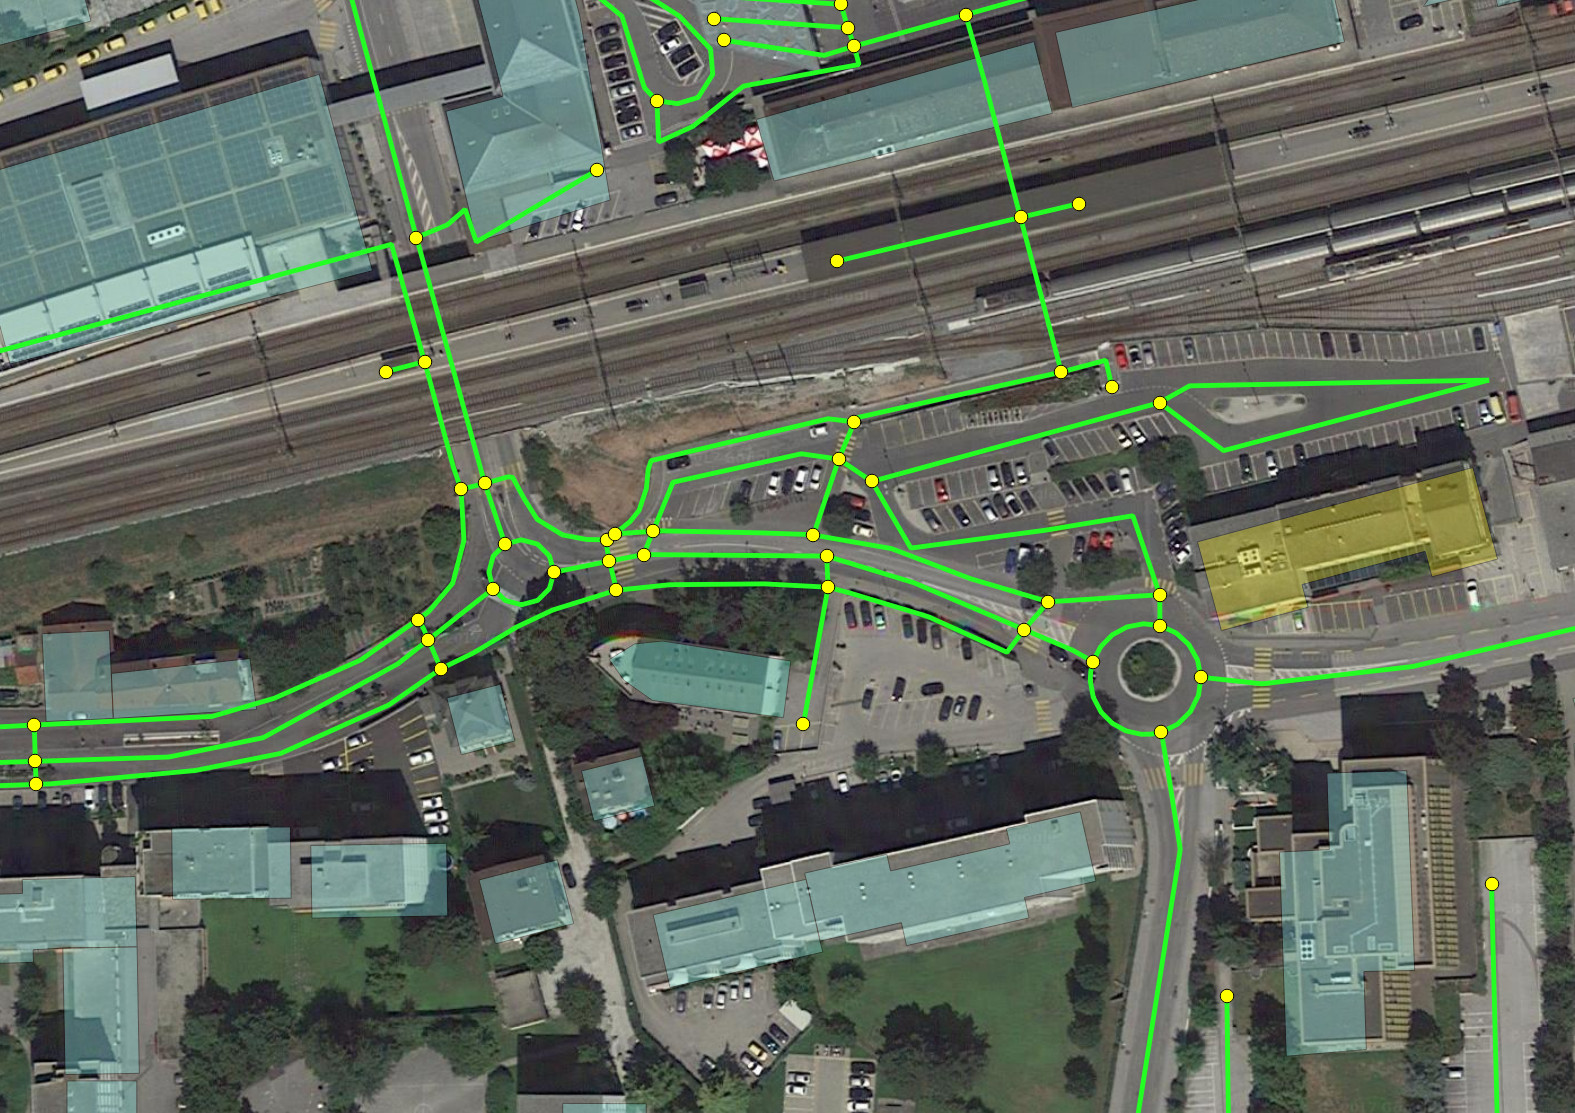
\includegraphics[width=1.0\linewidth]{OSM_walk_graph_02.jpg}
\end{center}
   \caption{Part of the pedestrian network extracted from OpenStreetMap (OSM) data (green) in a downtown area. On can clearly see that sidewalks information is not present everywhere. Background map: google satellite imagery. }\label{pedestriangraph}
\end{figure}

%################################################################################
%################################################################################
\section{Related work}
%################################################################################
%################################################################################
%This section will present the related work in the fields of each working packages.


%################################################################################
\subsection{Crowdsourcing}
%################################################################################
Crowdsourcing is the recent research field which focus on how to include people, mainly final-users, in the development and the design of a product \cite{ghezzi_crowdsourcing:_2017}. This may be game-oriented to maximize the number of crowd-workers and their motivation as well as to keep them participating as long as possible \cite{zeng_motivation_2017,morschheuser_gamified_2017}.

When data are collected by citizen, one talk about Citizen Science. If these data have a strong geospatial component, this lead to the field of Volunteered Geographic Information (VGI) \cite{sui_citizen_2013}. Brovelli et~al. \cite{brovelli_webbased_2014} and Minghini \cite{minghini_multi-dimensional_2014} shown how Participatory GIS using Free and Open Source Software (FOSS) may help providing high quality open-GIS data and making them available to the general public using web technologies. Brovelli et~al. \cite{brovelli_public_2016} also shown how VGI may improve urban monitoring and planing or tourism with mobile-based applications.\\

%\cite{hara_improving_2013} % bus stops
%\cite{hara_design_2016}
%\cite{kotaro_hara_projectsidewalk_nodate} % yt

In labeling tasks, some great care must be taken to maintain data quality. Gamification principles may be an invaluable help to keep users motivation and quality of their work \cite{von_ahn_labeling_2004,von2006peekaboom}. 

The OpenSideWalks project also takes benefits from Crowdsourcing \cite{noauthor_opensidewalks_nodate,tanweer_mapping_2017} to collect high quality open data. % opensidewalks

%\cite{association_for_computing_machinery_acm_tohme:_nodate} % yt


%################################################################################
\subsection{Computer Vision based techniques}
%################################################################################
Historically, CV tends to extract features from images like edges \cite{canny_computational_1986}.
Segmentation by watershed algorithms \cite{meyer_morphological_1990, beucher_segmentation:_1993} using graph-based techniques \cite{felzenszwalb_efficient_2004} or oriented gradient \cite{malisiewicz_ensemble_2011} gives the ability to well enough isolate regions on an image.
Hough transform is also a well know line detector that may be used to extract road boarders \cite{duda_use_1972,illingworth_survey_1988,ballard_generalizing_1981,kiryati_probabilistic_1991} as well as vanishing point extraction \cite{se_road_2003,wang2004lane,kong2009vanishing}.

Sky views are also known to provide good enough classification results, especially for crosswalks detection \cite{berriel_deep_2017}.

\cite{lu_real-time_2015} shows a simple approach to calculate the slope of a street by using lines which are known to be horizontal, like building windows edges.
%\cite{ivanchenko_crosswatch:_2008}
%\cite{asad_smartphone_2012}

It has already been shown \cite{hara_tohme:_2014, hara_design_2016} how CV was used to determine accessibility from physical features of the real world based on GSV. This approach is making use of ML techniques, especially Convolutional Neural Networks (CNN) which are typically designed to extract features from images \cite{lecun1995convolutional}. Field of autonomous driving brings a solid background for street segmentation using ML \cite{alvarez2012road}, even coupled with stereoscopic images which provides the useful depth information \cite{coughlan_terrain_2007,zbontar2016stereo}.
\cite{smith_classification_2013} used a more global approach coupled with a random forest classifier to identify sidewalks on street view images.

% \cite{association_for_computing_machinery_acm_tohme:_nodate} % yt



%################################################################################
\subsection{Coupling CS and CV algorithms to the DPLoS model}
%################################################################################
Level of Service (LoS) has long been studied for pedestrian (PLoS) \cite{landis_modeling_2001, gallin_quantifying_2001}. The former proposed a model that can help crossroads design and prioritize the needs for local governments. 

As sidewalks are probably the most important and secure places for pedestrian to walk on in urban areas, several studies have focused their researches on characterizing and assessing sidewalks accessibility.

\cite{tan_research_2007} compared the gap between the subjective security perception of pedestrian with traffic flow characteristics.

But it's rather new that a PLoS has been specifically investigated for disabled people (DPLoS). \cite{asadi-shekari_zohreh_disabled_2013} have for example calculated 10 main feature indicators. These indicators are themselves based on several studies and guidelines regarding facilities for disabled like wheelchair users or blind people. 
\cite{mostafavi2015mobilisig, gharebaghi2017confidence} focused on mapping the level of accessibility of street networks and \cite{liu_crowdsourcing-based_2017, comai_mapping_2015} on creating an accessibility mapping mobile application (MEP: Map for Easy Paths) using a user-centered design approach. 

\cite{coughlan_terrain_2007} and \cite{ivanchenko_computer_2008} used calculated depth map to detect negative obstacle edges on wheelchair users path by directly embedding a stereo camera onto the wheelchair. 

Other embedded based techniques make use of a smart-phone camera to detect crosswalk \cite{ivanchenko_crosswatch:_2008} or straight paths using CV and stereo vision \cite{asad_smartphone_2012}.

%A 2015 interdisciplinary urban data science program of the University of Washington \cite{rokem_building_2015} has seen 2 projects related to impaired people mobility. One of them, called 
OpenSideWalk \cite{bolten_urban_2015} investigated sidewalk graph analysis for routing to propose the better paths for disabled people. This project is now proposing a schema to better and more finely represents sidewalks as separate footways from the drivable roads in OpenStreetMap (OSM).%\footnote{\url{https://www.opensidewalks.com/}} \cite{noauthor_opensidewalks_nodate}.

Even the tourism industry may take some advantages of disabled accessibility researches \cite{israeli_preliminary_2002}.

%In Switzerland, one can easily find some architectural guidelines related to disabled pedestrians \cite{schmidt_directives_2003} mainly based on Swiss Standard (SN).

While \cite{kovashka2016crowdsourcing} addressed some of the most important questions regarding CV and CS and provide useful general guideline, it is only recently that DPLoS assessment or application design took advantages of CS and CV.
\cite{hara_feasibility_2012, comai_mapping_2015} have shown the opportunity of integrating final users in the design of an application devoted to disabled pedestrian and to assess scaled street segments aptitude.

Some of the most advanced studies \cite{hara_scalable_2014, hara_characterizing_2015} have shown how to combine CS and CV on Google Street View (GSV) images to collect informations on disabled pedestrians accessibility. The built tools \cite{hara_tohme:_2014} make use of Amazon Mechanical Turk (AMT) to achieve rapidly and at low cost some detection tasks on images. Recall of AMT workers combined with CV algorithms is higher and faster than AMT workers alone \cite{hara_combining_2013, hara_improving_2013, hara_improving_2015}. Thus, CV still endorse an important role in detecting features, especially when combined with ML.

The bottleneck in such approach is data acquisition and labeling. The latter is one of the highest time demanding operation. Thus, finding a pleasant way to annotate images with the highest quality is a key factor in this task \cite{von2006peekaboom}.


%################################################################################
%\subsection{Graph and network analysis}
%################################################################################
%\cite{boeing_osmnx:_2017}
%\cite{bolten_urban_2015}




%################################################################################
%################################################################################
\section{Proposed approach}
%################################################################################
%################################################################################
Based on the relevant literature, the research proposal is articulated in several phases.
Two first preliminary steps will be:
\begin{itemize}\setlength\itemsep{0.0em}
\item the creation of the DPLoS model and
\item the establishment of a pedestrian network at a city-scale level % (the city of Sion was chosen).
\end{itemize}  

Meanwhile, CV+ML algorithms dedicated to features detections in images will be settled together with dedicated CS applications to collect data, digitize and label features and evaluate the detection results.

These two steps must be closely related in their development as part of user inputs may influence CV+ML detection algorithms and algorithms results must be evaluated by crowd-workers and final users. 

%################################################################################
\subsection{DPLoS model}
%################################################################################
The DPLoS established model retains the 5 following features and value ranges: % set ranges here
\begin{itemize}
\item slope
\item sidewalks width and obstacles
\item coating quality (pavement, smooth concreet)
\item crosswalks and security signals (pedestrian light, refuge island)
\item presence of curb ramps to cross roads
\end{itemize}

%################################################################################
\subsection{Pedestrian graph}
%################################################################################
Existing vector data to establish the pedestrian graph may include National Map Agency (NMA) Cadastral Survey or vector data if available, OSM streets and footways or third party road networks.

\iffalse
\begin{itemize}\setlength\itemsep{0.0em}
\item National Map Agency (NMA) Cadastral Survey,
\item NMA vector data, if available or
%\item the Topographic Landscape Model (TLM) of the Federal Office of Topology, swisstopo,
\item OSM streets and footways
%\item any third party road network.
\end{itemize}
\fi

It is also conceivable to use high resolution satellite %or aerial raster 
data to extract a road network using segmentation-based classification methods
% but as this may involve more computational steps this solution was not chosen. They may however be an invaluable help to apply this method to 
in regions where high quality vector data does not exist. 

For this study, OSM street pathways data were extracted using a dedicated Python package \cite{boeing_osmnx:_2017}.


%################################################################################
\subsection{Crowdsourcing, Computer Vision and Machine Learning}
%################################################################################
%The development of an application, %even if located at later stage in the global process, 
%should be included as soon as possible. 
It was first decided not to use one, but rather 4 different stages depending on the goal to achieve. These goals are as follows:
\begin{enumerate}\setlength\itemsep{0.0em}
\item Footways network making of and update
\item Data acquisition: raw images + geolocation % and network segmentation
\item Images features digitizing and labeling %(on raw images)
\item End-user route choice and update abilities
\end{enumerate}

%#####################################
\subsubsection*{Footways network update}
%#####################################
The initial pedestrian network may not be totally fulfilled \ref{pedestriangraph}. It will be proposed as a Tool-as-a-Game (TaaG) to give crowd-workers a way to complete or make it fit the actual reality more precisely based on a recent orthophoto background. %This part may be desktop-oriented for a more comfortable data entry.


%#####################################
\subsubsection*{Data acquisition and geolocation + network segmentation}
%#####################################
The second stage, % which may be mobile-oriented 
would basically serve as a feeding source for raw images. 

Everyone can take a picture with a mobile device and upload it to a database. Along with existing street pictures sources like GSV or mapillary \cite{sweden_street-level_nodate,neuhold2017mapillary} %\footnote{\url{https://www.mapillary.com/}} \cite{sweden_street-level_nodate},
they will serve as raw data input for the digitizing step.
If a mobile GNSS receiver and a compass are enabled, geolocation values are stored along the picture. Otherwise, a geolocation tool will proposed to the user to geolocate and orient (azimuth) its photograph before uploading it. %A minimal precision will be asked for.\\



%#####################################
\subsubsection*{Feature digitizing and characterizing}
%#####################################
This third stage % could take benefits of larger screens, it will therefore be desktop-oriented. 
main goal is to digitize one or more of the 5 identified DPLoS features on raw images and marking them with attributes scores based on the DPLoS model. 

E.g., if someone sees a curb ramp on a picture, he will be able to digitize it and marking it as a curb ramp \ref{curbramppicture}. An other example would let the user annotate a sidewalk surface width as %"not crossable for two wheelchairs" or 
"no possible way for a single wheelchair" based on the perceived width on the given picture. If depth information is available %for an image, 
a measuring tool may also be provided.

\begin{figure}[ht]
\begin{center}
%\fbox{\rule{0pt}{2in} \rule{0.9\linewidth}{0pt}}
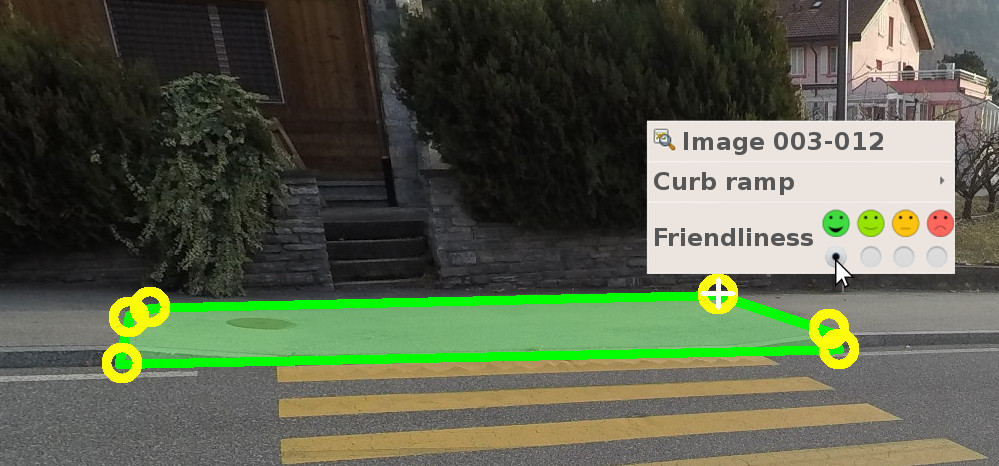
\includegraphics[width=1.0\linewidth]{curb_ramp.jpg}
\end{center}
   \caption{An example on digitizing a curb ramp on a picture. }\label{curbramppicture}
\label{fig:long}
\label{fig:onecol}
\end{figure}

This second application will also give the user a TaaG to check the features that were detected by algorithms. This important step provides two advantages:
\begin{enumerate}\setlength\itemsep{-0.0em}
\item it will classify detected features according to a confusion matrix \ref{confmat}.

%\iffalse
\vspace*{-0.0em}
\begin{table}[ht]
\caption{Confusion matrix}\label{confmat}
%\resizebox{0.5\textwidth}{!}{%
\setlength\tabcolsep{12pt}
\begin{tabular}{ l r c c }
%\toprule
\multicolumn{2}{ c }{} & \multicolumn{2}{ c }{{Detection} } \\
%\addlinespace
\cmidrule{3-4}
& & \makecell{{Positive}} & \makecell{{Negative}} \\
\cmidrule{3-4}
\multirow{2}{*}[0.2em]{\raisebox{4em}{\rotatebox[origin=c]{90}{Ground}~\rotatebox[origin=c]{90}{truth}}} & \makecell{Positive} & {True positive} & {False negative}  \\ 
 & \makecell{Negative} & False positive & True negative \\ 
\cmidrule{3-4}
%\bottomrule
\end{tabular}
%}
\end{table}	
%\fi

\item ML detection algorithms abilities could be improved by feeding them back these new positive and negative labeled images for a new training. Training results must be tracked to avoid overfitting.
\end{enumerate}




%#####################################
\subsubsection*{End-user route choice and update}
%#####################################
The last application will target the impaired pedestrian street users. It will propose the best route between two points based on the better DPLoS edges as define by eq.\,\ref{dplostot}.
\begin{equation}
\mathrm{DPLoS}_{\mathit{route}} = \frac{1}{n}\sum{\mathrm{DPLoS}_{n\cdot\mathit{segment}}}
\label{dplostot}
\end{equation}


An additional tab will offer the user the possibility to give its feedback on a selected segment, for example when he sees an inadequate between the real world and a feature on the segment. This will improve the pedestrian network and update it as urban environment is changing.




%################################################################################
%\subsection{Computer Vision and Machine Learning}
%################################################################################




%################################################################################
%################################################################################
%\section{Preliminary Results and Evaluation}
%################################################################################
%################################################################################




%################################################################################
%################################################################################
\section{Conclusion and future work}
%################################################################################
%################################################################################
This project is in its early stages. The first version of the DPLoS model is ready. The setting up of a database to store images metadata like geolocation, as well as algorithms and crowd-workers labeling results is taking place. This same database will serve the four different applications through APIs that need to be developed. It will finally need further investigating and tests regarding coupling of CV and ML algorithms. Database populating and labeling will be the most resource demanding tasks.




%################################################################################
%################################################################################
%\section*{Acknowledgement}
%################################################################################
%################################################################################



%%%%%%%%%%%%%%%%%%%%%%%%%%%%%%%%%%%%%%%%%%%%%%%%%%%%%%%%%%%%%%%%%%%%%%%%%%%%%%%%

\bibliographystyle{./myIEEEtran}
%\nocite{*} 
\bibliography{biblio}

\end{document}
